% ============================
% Section: Case Application - 90Y Microsphere Therapy
% ============================

\label{sec:case}

To illustrate the usefulness and problems of PET/MR a case application is presented. The comparison of PET/CT and PET/MRI for post-therapy quantitative imaging of Yttrium-90 (90Y) distribution given by Knesaurek et al. \cite{knesaurek2018} is followed.

Yttrium-90 (90Y) microsphere therapy, also known as Selective Internal Radiation Therapy (SIRT) %Underscored SIRT
, is an emerging treatment for unresectable hepatic tumors. This therapy delivers targeted radiation with microspheres loaded with 90Y with the objective of spare healthy tissues and concentrate the dose within tumors.

Although both techniques offer information on tumor dosimetry, their unique benefits and drawbacks must be carefully considered before being used in clinical settings. This section explores imaging parameters, dosimetry results, and tumor delineation findings, with a focus on their implications for radiotherapy planning and outcomes.

In Knesaurek et al.’s prospective study, 32 patients underwent sequential imaging on a PET/CT system and a PET/MR system immediately following 90Y-SIRT. The PET/CT acquisition used a Siemens Biograph mCT system with time-of-flight (TOF) capabilities and low-dose CT scans were employed for attenuation correction. PET/MR imaging was performed using a Siemens Biograph mMR system, which uses avalanche photodiodes (APDs) instead of photomultiplier tubes but lacks TOF capabilities. 
Attenuation correction for PET/MR relied on four-tissue segmentation derived from Dixon sequences, %Needs explanation how?
to compensate for the lack of CT-based corrections. Imaging parameters included matrix size, voxel sizes and acquisition times. 

%wrote: Not SBRT...

Both modalities implemented advanced reconstruction algorithms: Poisson-ordered subset expectation maximization (OP-OSEM3D) with TOF and point spread function (PSF) for PET/CT, and OP-OSEM3D with PSF for PET/MR. Validation was conducted through a phantom study using a 90Y-filled Jaszczak sphere, that ensured cross-calibration and consistency in dosimetry across the systems.

%Knešaureks Fig. 1 | Phantom study comparing PET/CT and PET/MRI for 90Y calibration
% visually support system calibration.

Figure \ref{fig:phantom_petct_petmri} demonstrates the results of that phantom study, it compares PET/CT and PET/MRI systems for $^{90}\text{Y}$ calibration. Results indicate that both systems are closely calibrated for \(^{90}\text{Y}\) with less than 1\% difference.

\begin{figure*}[ht]
	\centering
	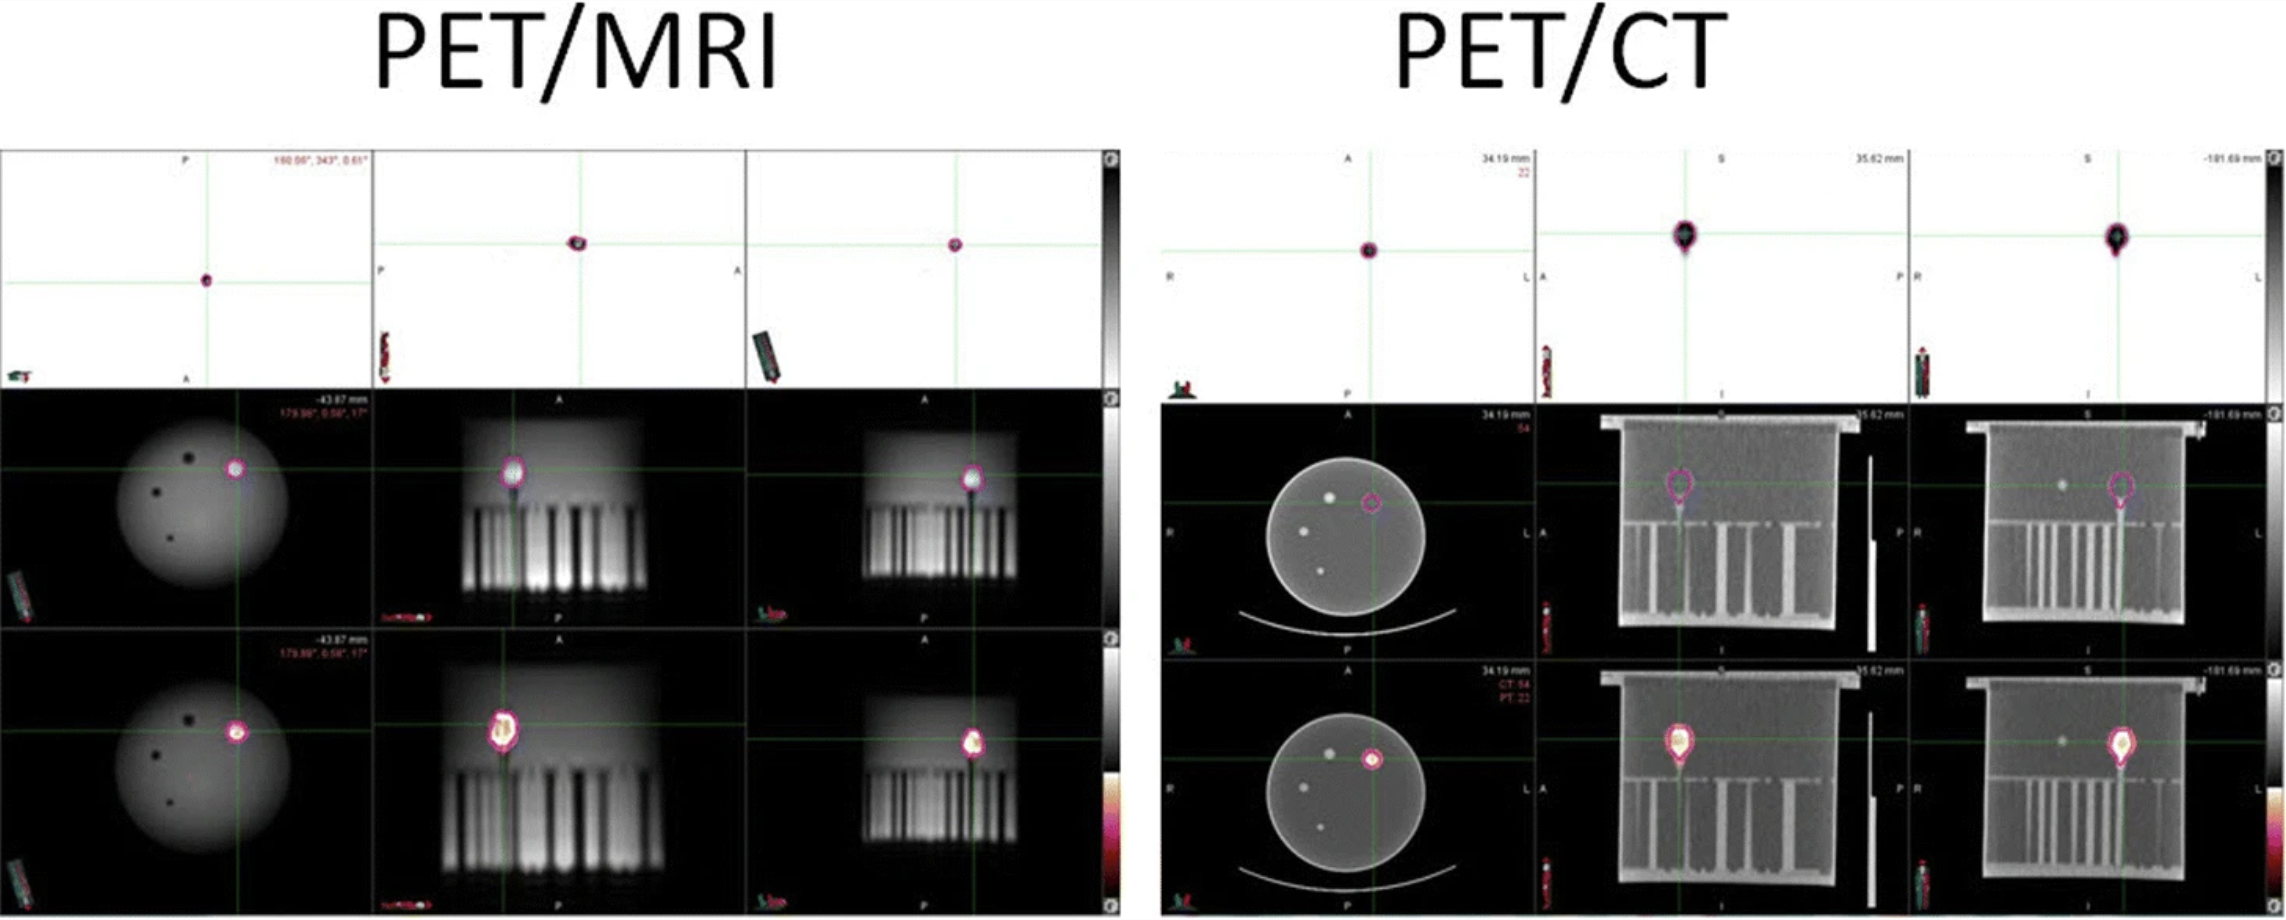
\includegraphics[width=0.9\textwidth]{assets/PETCT_vs_PETMRI_Phantom.png} % Replace with the correct file path
	\caption{Phantom study comparing PET/CT and PET/MRI for \(^{90}\text{Y}\) calibration. The top row displays PET images, the middle row shows MRI and CT images respectively, and the bottom row presents fused PET/MRI and PET/CT images.  Adapted from Knešaurek et al. \cite{knesaurek2018}.}
	\label{fig:phantom_petct_petmri}
\end{figure*}

This methodology provides a foundation for analyzing tumor delineation, motion management, soft-tissue contrast, and dosimetric accuracy between PET/CT and PET/MR. The following sections discuss these aspects.

\subsubsection{Target delineation}

\paragraph{Image Registration and Fusion.} 

PET/CT simultaneous acquisition ensure spatial consistency across datasets \cite{TG132}. This simplifies radiotherapy planing, particularly in workflows that require direct integration into treatment planning systems. 

PET/MR relies on deformable image registration to align PET data with MR images, as the datasets are acquired using different mechanisms and frames of reference. % needs explanation

The challenge here are the errors produced by differences on the anatomy contrast and the distortions from MRI technique.

Knesaurek et al. \cite{knesaurek2018}, exemplifies this with the need to implement and use a vast collection of MRI sequences for delineation and creation of tumor ROIs. 

%revise
\paragraph{Motion Management}

There are different approaches to address motion artifacts during the acquisition of the images, for liver cancer is significant because of its location near the diaphragm. PET/CT relies on gated acquisition or time-weighted averaging methods to account for motion blur, but these methods are limited in capturing the full range of liver motion \cite{Dhont2020}. 

PET/MR offers an advantage as it can see motion during PET with MR motion correction sequences %wrote ? underscored MR motion correction sequences
aiding in reconstruction and reducing artifacts\cite{knesaurek2018}. Dhont et al. \cite{Dhont2020} noted that motion-resolved PET/MR provides better tumor localization and volume estimation for motion-prone tumors, potentially improving dose escalation accuracy.

Applying motion correction techniques, %How is this done?
such as those available in PET/MRI systems, could mitigate these effects and improve reliability in T/N ratio calculations \cite{knesaurek2018}. This is particularly important in cases where respiratory motion introduces artifacts, as shown in Figure \ref{fig:respiratory_motion_artifacts}, which demonstrates $^{90}\text{Y}$ spillover into the lungs during PET/CT imaging due to diaphragm motion.

%Knešaureks Fig. 4 | Respiratory motion artifacts and spillover with 90Y
%	Relevant if discussing motion artifacts

\begin{figure*}[ht]
	\centering
	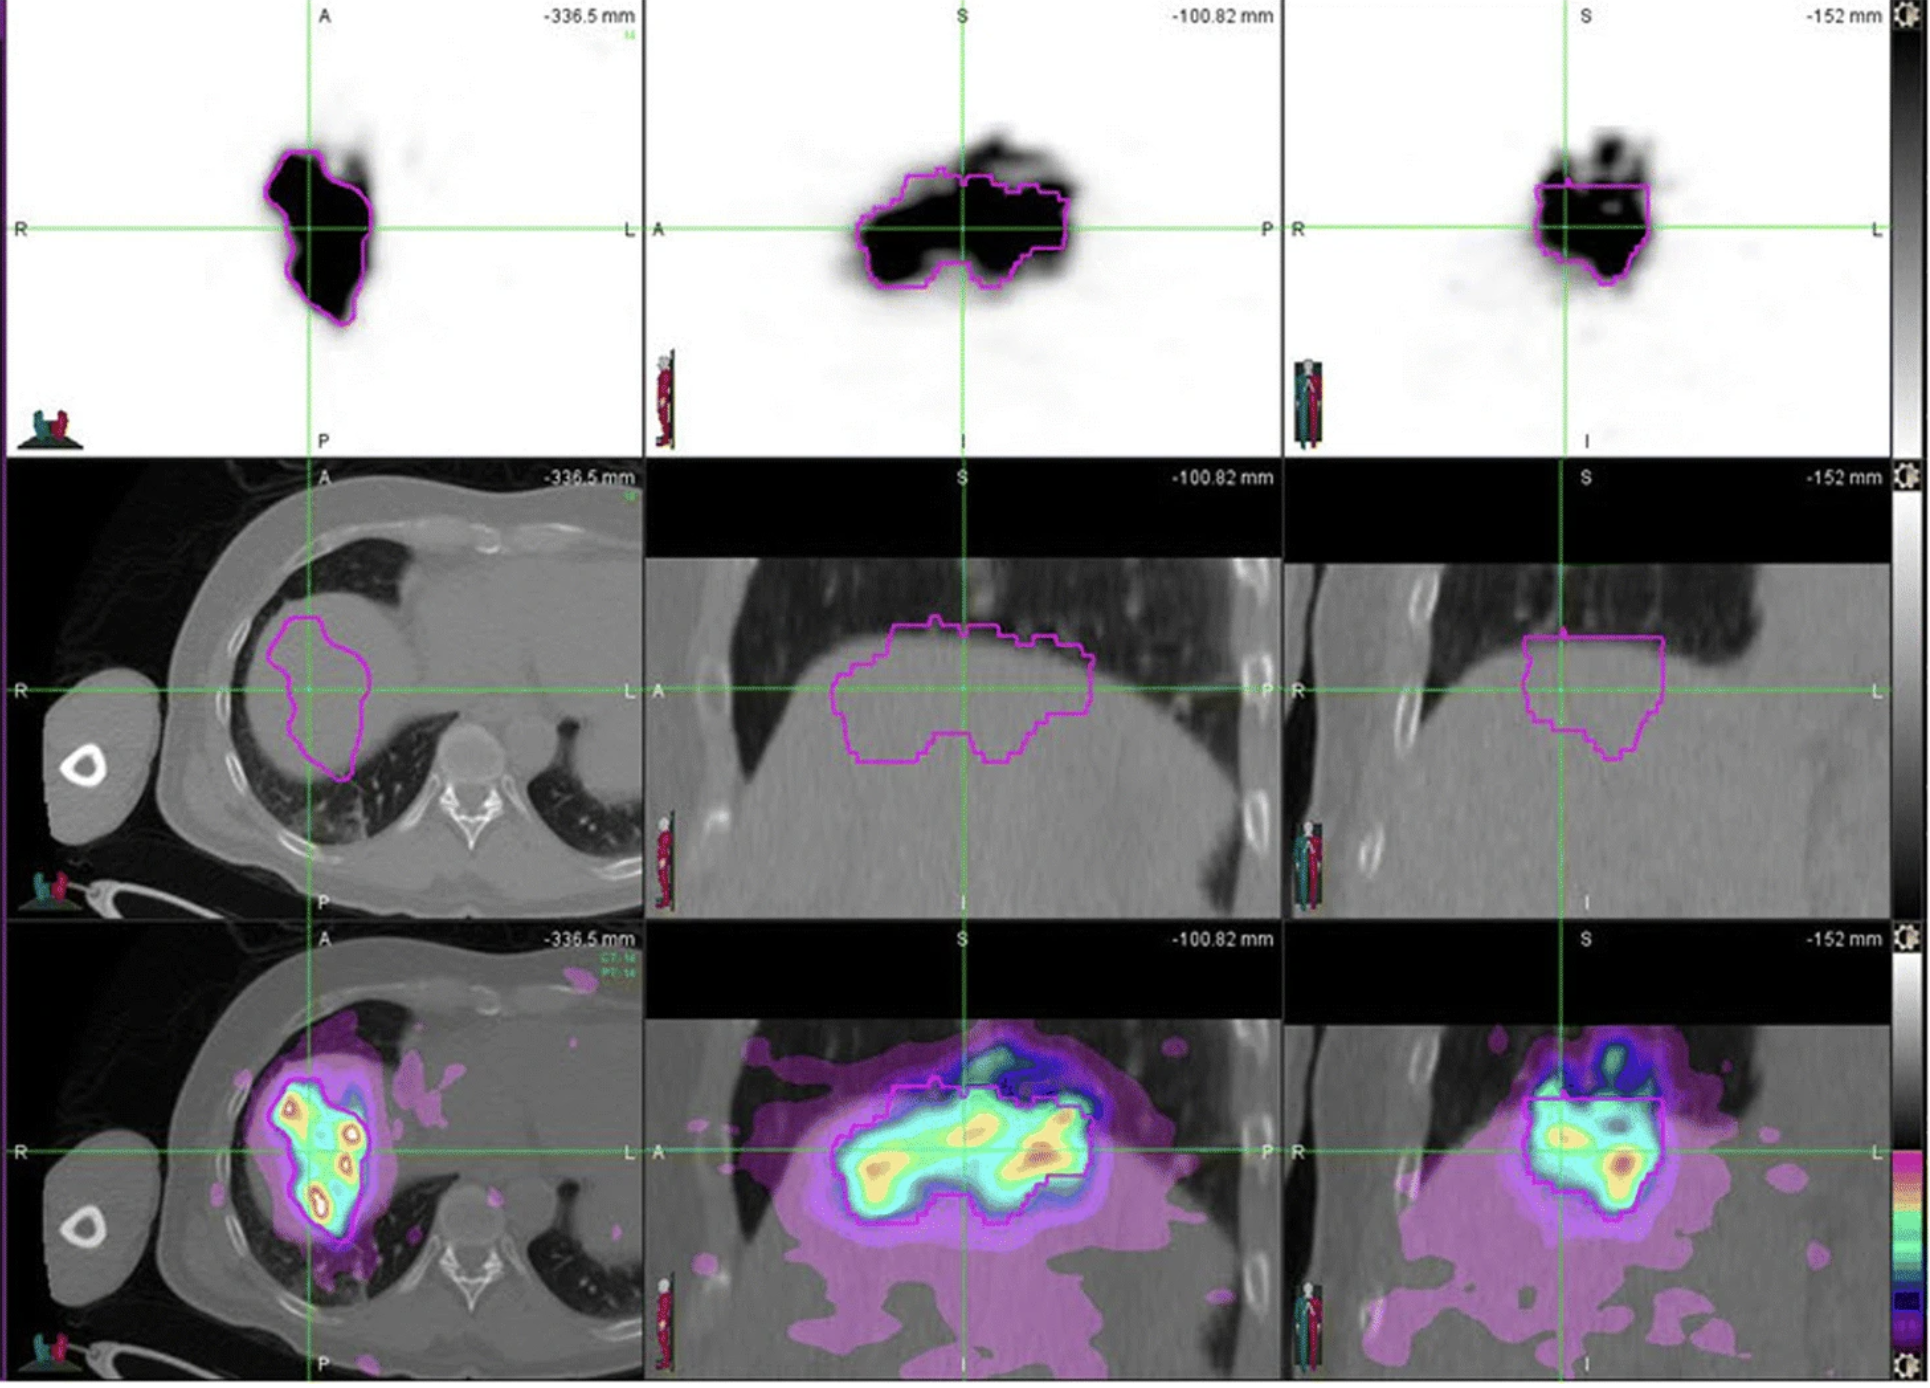
\includegraphics[width=0.9\textwidth]{assets/Respiratory_Motion_Artifacts.png} 
	\caption{Respiratory motion artifacts and spillover with \(^{90}\text{Y}\) imaging using PET/CT. The top row displays uncorrected PET images in axial (left), sagittal (middle), and coronal (right) views. The middle row shows the corresponding CT anatomical references, and the bottom row presents fused PET/CT images, where spillover into the lungs due to respiratory motion is evident. Adapted from Knešaurek et al. \cite{knesaurek2018}.}
	\label{fig:respiratory_motion_artifacts}
\end{figure*}



\paragraph{Soft-Tissue Contrast}

The most significant advantage of PET/MR lies in soft-tissue contrast, with proper contrast comes better differentiation of liver tumors from healthy tissue and surrounding structures:

PET/MR is particularly effective for delineation small liver tumors ($<$2 cm), where partial volume effects in PET/CT can compromise visualization. \cite{knesaurek2018} Also it is demonstrated that ROIs derived from MR images allow more precise tumor targeting in challenging cases, such as when tumors are indistinct in CT. %wrote Liver? SBRT?


\paragraph{Acquisition Time and Workflow}

The total acquisition time for PET/CT is largely determined by the PET component, as CT acquisition takes only seconds. This efficiency makes PET/CT the preferred choice for high-throughput settings\cite{knesaurek2018}.
While in PET/MR, acquisition time is dictated by the MR component, which can significantly increase scan duration due to the need for multiple MR sequences. %why?
While this trade-off is justified for cases requiring detailed anatomical or functional imaging, it limits PET/MR’s utility in busy clinical workflows \cite{knesaurek2018}.

%wrote in general for this page moslty surface description without significant development on physics or clinical
%lots of material & opportunities to explain the physics / tecnical / approach in detail

\subsubsection{Dosimetry}
At the end a solid argument to be made in favor of an imaging technique for treatment planning revolves around dosimetry. Dosimetry impacts treatment efficacy and seeks to minimize damage to healthy tissue. The main differences between PET/CT and PET/MR reside on their technical characteristics leading to distinct applications and limitations.

\paragraph{Attenuation Correction and Quantitative Accuracy.}

The fact that PET/CT are a single system is a huge advantage as CT provides attenuation correction. More reliable SUV values and dose calculations will result from the high-density resolution of CT all this while having a reproducible attenuation correction across a wide range of tissues

The MR attenuation correction is less accurate, the lack of direct bone density mapping may lead to underestimation of attenuation in osseous structures on the surrounding areas. Moreover, MR AC requires segmentation of tissues into predefined classes (e.g., air, soft tissue, fat, bone). Liver cancer imaging often deals with heterogeneous structures (e.g., cirrhotic livers, metastases). Errors in segmentation directly impact ROI creation and subsequent dosimetry calculations. 


Following the work of Knesaurek, \cite{knesaurek2018} PET/CT typically provides slightly higher SUVmean and SUVmax values compared to PET/MR, which may lead to discrepancies in tumor delineation and dosimetry calculations. The mean liver dose for $^{90}\text{Y}$ therapy was 51.6 Gy with PET/CT and 46.5 Gy with PET/MR, with differences attributed to variations in attenuation correction and liver volume estimation.

%figure 4 is way down may shift once following sections are done
Figure \ref{fig:patient_liver_dose} shows the liver dosimetry differences between PET/CT and PET/MRI in a patient study. It is important to notice the variations in attenuation correction and liver volume estimation. The mean liver dose obtained from PET/CT was 38.81 Gy, while PET/MRI measured 31.64 Gy, with differences attributed to variations in attenuation correction and liver volume estimation.

%Knešaureks Fig. 2 | Patient study with highest mean liver dose difference
%highlight liver dosimetry differences.
\begin{figure*}[ht]
	\centering
	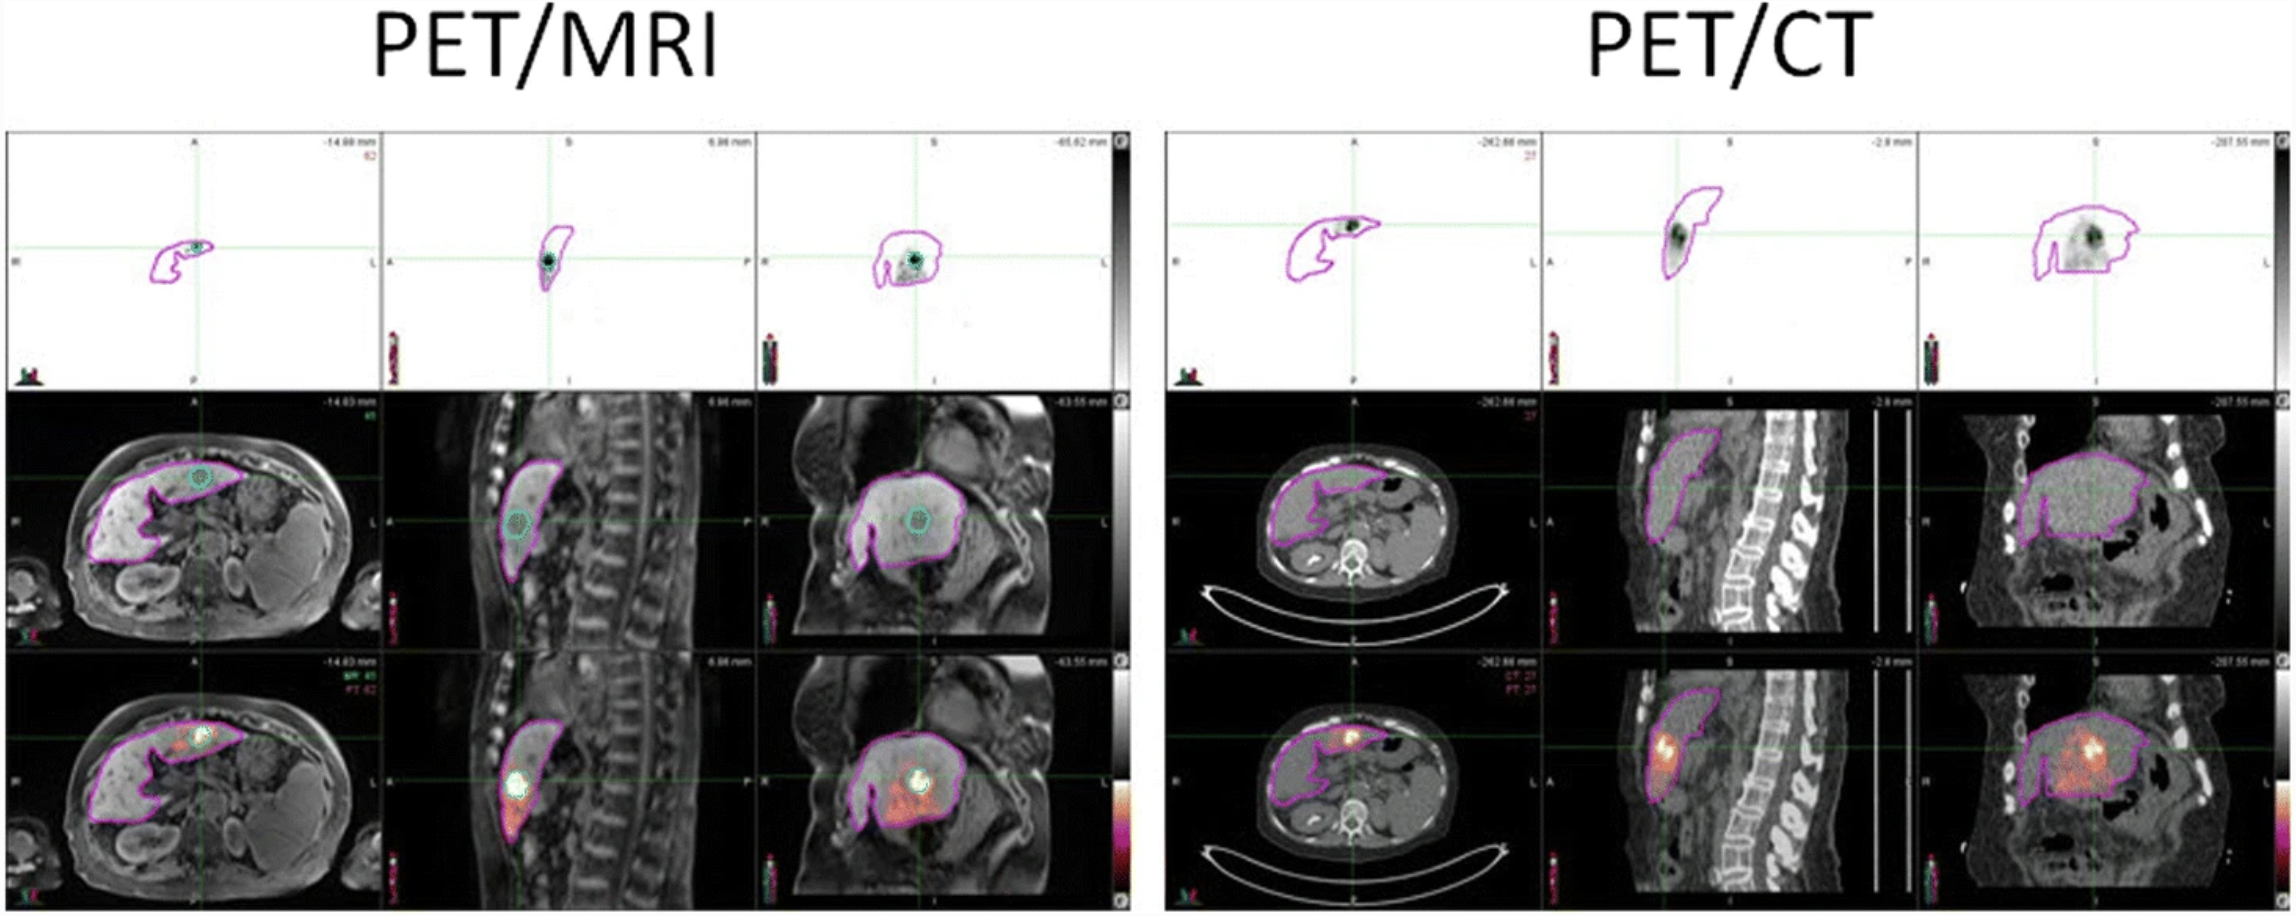
\includegraphics[width=0.9\textwidth]{assets/Liver_Dosimetry_Differences.png} 
	\caption{Patient study showing the highest mean liver dose difference between PET/CT and PET/MRI. The top row displays PET images, the middle row shows MRI and CT images respectively, and the bottom row presents fused PET/MRI and PET/CT images. Adapted from Knešaurek et al. \cite{knesaurek2018}.}
	\label{fig:patient_liver_dose}
\end{figure*}

\paragraph{Partial Volume Effects}

Both PET/CT and PET/MR suffer from the imaging limitation of Partial volume effects (PVE). It occurs due to signal averaging across tissue borders inside a voxel. Then, tasks like tumor segmentation become more difficult as a result of the blurring edges and decreased precision in defining volumes of interest. 

PET/CT has a broad field of view and good tumor-to-node contrast, but its poorer spatial resolution and vulnerability to PVE make it difficult to quantify since they can cloud tumor borders. Fortunately PET/MRI can be utilized to correct PVE in PET pictures because of MRI's higher soft-tissue contrast and great spatial resolution. 

Knesaurek et al. \cite{knesaurek2018} reported that partial volume effects (PVEs) significantly impact quantification and dosimetry calculations, particularly for small tumors. Both modalities analyzed a tumor volume of approximately 7.0 $\text{cm}^3$ and mentions no use of contrast media. Intra hepatic dosimetry calculations of T/N ratios, requires using of contrast in anatomical modalities, as well as,
PV corrections for lesions smaller than 2.5 $\text{cm}$. And respiratory motion contributes the challenge of accurate T/N ratio estimation for undersized lesions, also noticible in figure \ref{fig:respiratory_motion_artifacts}.

\paragraph{Tumor-to-Normal Tissue Ratios (T/N Ratios)}

Thanks to soft-tissue contrast, which aids in more precise tumor delineation, PET/MR will have a higher T/N ratio. In organs like the liver this should be a requirement in order to spare and distinguish tumors from healthy liver tissue or adjacent structures.


On the other hand, PET/CT has the benefit of more precise attenuation correction, allowing for more accurate dose estimations and standardized uptake value (SUV) calculations. However, its accuracy in detecting tiny tumor boundaries gets limited by its poorer soft-tissue contrast as compared to PET/MR, especially when no contrast medium is present. This displays the way PET/MR can be preferable when dealing with complicated anatomy, such as the liver, by offering better distinction.


Knesaurek et al. \cite{knesaurek2018} managed to calculate T/N ratios for the PET/CT scan by leveraging MRI-derived tumor ROIs merged with CT images through deformable transformation, a process that aligns images from different modalities to a common coordinate system, in MIM software. The study reported T/N ratios of 24.90 for PET/CT and 30.00 for PET/MRI. 

Additionally, the absence of contrast agents in both CT and MRI images likely reduced the accuracy of tumor delineation and intra-hepatic dosimetry. The findings highlight the potential of PET/MRI to achieve superior T/N ratios (delivering higher relative doses to tumor regions), but also emphasize the importance of integrating advanced techniques like PVE corrections, contrast agents, and motion management into dosimetric workflows for small liver tumors.

